\documentclass[compress,trans,9pt]{beamer}
% \documentclass[9pt]{beamer}
%\documentclass[compress,9pt,usenames,dvipsnames]{beamer}
% \usepackage[utf8]{inputenc}
% \includeonlyframes{current}
\input{Common}

\begin{document}

\AtBeginSection[]
  {
     \begin{frame}<beamer>
     \frametitle{Plan}
     \tableofcontents[currentsection]
     \end{frame}
  }


%-------------- start slide -------------------------------%{{{
\begin{frame}[noframenumbering]
  \titlepage
\end{frame}
%-------------- end slide -------------------------------%}}}


% \begin{frame}{Outline}
%   \tableofcontents
%   % You might wish to add the option [pausesections]
% \end{frame}

\newcommand{\myChapter}{Chapter 6. Hypothesis Testing}

%-------------- start slide -------------------------------%{{{
\begin{frame}
\begin{center}
\huge
\myChapter
\end{center}
\end{frame}
%-------------- end slide -------------------------------%}}}
\mySection{6.1 Introduction}
%-------------- start slide -------------------------------%{{{ 6.4
\begin{frame}
Instead of numerical estimates of parameters, in the form of either single points or confidence intervals, we want to make a choice between two conflicting theories, or {\bf hypothesis}:
\pause
\vfill
\begin{enumerate}
 \item $H_0$: the null hypothesis
 \item[] \hspace{3em} v.s.
 \item $H_1$: the alternative hypothesis
\end{enumerate}
\pause
\vfill
Comments:
\underline{Hypothesis testing} and \underline{confidence intervals} are dual concepts to each other:
\begin{itemize}
	\item One can be obtained from the other.
	\item However, it is often difficult to specify $\mu_0$ to the null hypothesis.
\end{itemize}
\end{frame}
%-------------- end slide -------------------------------%}}}


\mySection{6.2 The Decision Rule}
%-------------- start slide -------------------------------%{{{ 1
\begin{frame}[fragile]
 \begin{center}
 \begin{minipage}{0.6\textwidth}
 \begin{center}
Go over the example first....
\end{center}
 \end{minipage}
\end{center}
\end{frame}
%-------------- end slide -------------------------------%}}}
%-------------- start slide -------------------------------%{{{ 1
\begin{frame}[fragile]
 \begin{center}
 \begin{minipage}{0.6\textwidth}
 \begin{center}
    Suppose our friend Jory claims that he has some magic power to predict the side of a randomly tossed fair-coin.
    \bigskip

    Jory claims that he could do more than\\ $\textcolor{magenta}{1/2}$ \\ of the time on average.
    \bigskip

    Let's test Jory to see if we believe his claim.
\end{center}
 \end{minipage}
\end{center}
\end{frame}
%-------------- end slide -------------------------------%}}}
%-------------- start slide -------------------------------%{{{ 1
\begin{frame}[fragile]
 \begin{center}
 \begin{minipage}{0.6\textwidth}
 \begin{center}
    We made Jory guess a repeatedly tossed coin for 100 times.
    \bigskip

    He guesses correctly 54 times.
    \bigskip
    \bigskip

    {\bf  Question: }\\

    Does this provide strong evidence that Jory has the proclaimed magic power?
\end{center}
 \end{minipage}
\end{center}
\end{frame}
%-------------- end slide -------------------------------%}}}
%-------------- start slide -------------------------------%{{{ 1
\begin{frame}[fragile]
 \begin{center}
 If Jory is guessing randomly,  the number of correct guesses would follow a binomial distribution
 with parameters $n=100$ and $p=1/2$.
 \bigskip
 \bigskip

\includegraphics[scale=0.4]{Codes/Binomial_Jory.png}

\end{center}

\end{frame}
%-------------- end slide -------------------------------%}}}
%-------------- start slide -------------------------------%{{{ Guess 54
\begin{frame}[fragile]
\def\guess{54}
\def\ans{0.2421}
  \begin{center}
    What is probability that Jory gets \textcolor{red}{\guess\: or more} correct when guessing randomly?
 \bigskip
  \pause

 \includegraphics[scale=0.4]{Binomial_Jory_\guess.png}
  \end{center}
\bigskip
\begin{align*}
  \bbP\left(X\ge \guess\right) = \sum_{n=\guess}^{100} \binom{100}{n} \left(\frac{1}{2}\right)^n \left(\frac{1}{2}\right)^{100-n} = \textcolor{red}{\ans}.
\end{align*}
 \end{frame}
%-------------- end slide -------------------------------%}}}
%-------------- start slide -------------------------------%{{{ 54: Conclusion
\begin{frame}[fragile]
 \begin{center}
 \begin{minipage}{0.6\textwidth}
 \begin{center}
  It is not unlikely to get this many correct guesses due to chance.

  \bigskip
  \bigskip

  {\bf Conclusion:}\\
  \bigskip

  There is No strong evidence that Jory has better than a $1/2$ chance of correctly guessing the coin.

\end{center}
 \end{minipage}
\end{center}
\end{frame}
%-------------- end slide -------------------------------%}}}
%-------------- start slide -------------------------------%{{{ Guess 60
\begin{frame}[fragile]
\def\guess{60}
\def\ans{0.0284}
  \begin{center}
    What is probability that Jory gets \textcolor{red}{\guess\: or more} correct when guessing randomly?
 \bigskip
  \pause

 \includegraphics[scale=0.4]{Binomial_Jory_\guess.png}
  \end{center}
\bigskip
\begin{align*}
  \bbP\left(X\ge \guess\right) = \sum_{n=\guess}^{100} \binom{100}{n} \left(\frac{1}{2}\right)^n \left(\frac{1}{2}\right)^{100-n} = \textcolor{red}{\ans}.
\end{align*}
 \end{frame}
%-------------- end slide -------------------------------%}}}
%-------------- start slide -------------------------------%{{{ 60: Conclusion
\begin{frame}[fragile]
 \begin{center}
 \begin{minipage}{0.6\textwidth}
 \begin{center}
 Either
 \bigskip

\textcolor{red}{Jory is purely guessing with probability of success of $\frac{1}{2}$, and we witnessed a very unusual event due to chance.}

  \bigskip \pause
  Or
  \bigskip

  \textcolor{green}{ Jory is truly having the magic power to guess the coin.}
  \bigskip \pause

\mySeparateLine

{\bf Conclusion:}\\[1em]

We have strong evidence against \\
\textcolor{red}{Red Hypothesis} \\[1em]

Or the test is in favor of \\
\textcolor{green}{Green Hypothesis}


% that Jory does have the magic power to do better than a $1/2$ chance of correctly guessing the coin.

\end{center}
 \end{minipage}
\end{center}
\end{frame}
%-------------- end slide -------------------------------%}}}
%-------------- start slide -------------------------------%{{{ 1
\begin{frame}[fragile]
 \begin{center}
 \begin{minipage}{0.6\textwidth}
 \begin{center}
  Before testing Jory, could you set up a threshold above which we will believe Jory's super power?
  \bigskip
  \pause

  Find smallest $\textcolor{red}{m}$ such that

\begin{align*}
  \bbP\left(X\ge \textcolor{red}{m}\right) = \sum_{n=\textcolor{red}{m}}^{100} \binom{100}{n} \left(\frac{1}{2}\right)^n \left(\frac{1}{2}\right)^{100-n} \le \textcolor{red}{0.05}
\end{align*}
\pause
\[\Downarrow\]
\begin{align*}
\boxed{m = 59}
\end{align*}
\small
b.c. $\bbP\left(X\ge 58\right)=0.067$ \& $\bbP\left(X\ge 59\right)=0.044$
  \end{center}
 \end{minipage}
\end{center}
\end{frame}
%-------------- end slide -------------------------------%}}}
%-------------- start slide -------------------------------%{{{ 1
\begin{frame}[fragile]
 \begin{center}
 \begin{minipage}{0.6\textwidth}
 \begin{center}
 We have just informally conducted a hypothesis test with the\\
 \textcolor{red}{null hypothesis}
 \begin{align*}
   \textcolor{red}{H_0: p=\frac{1}{2}}
 \end{align*}
 against the \\
 \textcolor{green}{alternative hypothesis}
 \begin{align*}
   \textcolor{green}{H_1: p>\frac{1}{2}}
 \end{align*}
 under the\\
 \textcolor{yellow}{significance level $\alpha=0.05$}\\[0.5em]
 which is equivalent to either \\[1em]
 \begin{minipage}{0.45\textwidth}
 \begin{center}
 producing the \\
 \textcolor{yellow}{critical region\\
 $m\ge 59$}
 \end{center}
 \end{minipage}
 \hfill or \hfill
 \begin{minipage}{0.45\textwidth}
 \begin{center}
 comparing with \\
 the \textcolor{yellow}{p-value.}
 \end{center}
 \end{minipage}
 \end{center}
 \end{minipage}
\end{center}
\end{frame}
%-------------- end slide -------------------------------%}}}
%-------------- start slide -------------------------------%{{{ 6.8
\begin{frame}
\begin{itemize}
  \item  \textcolor{magenta}{Test statistic:}
		Any function of the observed data whose numerical value
		dictates whether $H_0$ is accepted or rejected.
	\vfill
  \item  \textcolor{magenta}{Critical region} $C$:
		The set of values for the test statistic that result in
		the null hypothesis being rejected.\\[1em]
  \item[] \textcolor{magenta}{Critical value}:
		The particular point in $C$ that separates the rejection region from the acceptance region.
	\vfill
   \item \textcolor{magenta}{Level of significance} $\alpha$:
		The probability that the test statistic lies in the critical region $C$ under $H_0$.
\end{itemize}
\end{frame}
%-------------- end slide -------------------------------%}}}
%-------------- start slide -------------------------------%{{{ 6.9
\begin{frame}{Test Normal mean $H_0: \mu=\mu_0$ ($\sigma$ known)}

{\bf Setup:~}
\begin{enumerate}
 \item Let $Y_1=y_1,\cdots,Y_n=y_n$ be a random sample of size $n$ from $N(\mu,\sigma^2)$ with $\sigma$ known.
  \item Set $\bar{y}=\frac{1}{n}(y_1+\cdots+y_n)$ and $z=\frac{\bar{y}-\mu_0}{\sigma/\sqrt{n}}$.
 \item The level of significance is $\alpha$.
\end{enumerate}

\vfill\pause
{\bf Test:}\\
\begin{minipage}{0.3\textwidth}
 \[
 \begin{cases}
     H_0: \mu= \mu_0 \\
     H_1: \mu> \mu_0 \\
 \end{cases}
 \]
 reject $H_0$ if $z\ge z_\alpha$.
\end{minipage}
\hfill
\begin{minipage}{0.3\textwidth}
 \[
 \begin{cases}
     H_0: \mu= \mu_0 \\
     H_1: \mu< \mu_0 \\
 \end{cases}
 \]
 reject $H_0$ if $z\le -z_\alpha$.
\end{minipage}
\hfill
\begin{minipage}{0.3\textwidth}
 \[
 \begin{cases}
     H_0: \mu= \mu_0 \\
     H_1: \mu\ne \mu_0 \\
 \end{cases}
  \]
  reject $H_0$ if $|z|\ge z_{\alpha/2}$.
\end{minipage}
\end{frame}
%-------------- end slide -------------------------------%}}}
%-------------- start slide -------------------------------%{{{ 6.10
\begin{frame}
\begin{itemize}
  \item \textcolor{magenta}{Simple hypothesis}: Any hypothesis which specifies the population distribution completely.\\[1em]
  \item \textcolor{magenta}{Composite hypothesis}: Any hypothesis which does not specify the population distribution completely. \\[2em]
	\item[Conv.] We always assume $H_0$ is simple and $H_1$ is composite.
\end{itemize}

\end{frame}
%-------------- end slide -------------------------------%}}}
%-------------- start slide -------------------------------%{{{ 6.11
\begin{frame}

{\bf Definition.~} The \textcolor{magenta}{P-value} associated with an observed test statistic is the
probability of getting a value for that test statistic as extreme as or more
extreme than what was actually observed (relative to $H_1$) given that $H_0$ is
true.
\pause
% \vspace{2em}
% Comments.
% \begin{itemize}
%  \item
% \item
% \end{itemize}
\vfill
Note: Test statistics that yield small P-values should be interpreted as evidence
against $H_0$.
\vfill
\pause
\begin{enumerate}
 \item[E.g. ] Suppose that test statistic $z=0.60$. Find P-value for
 \begin{minipage}{0.3\textwidth}
 \[
 \begin{cases}
     H_0: \mu= \mu_0 \\
     H_1: \mu> \mu_0 \\
 \end{cases}
 \]
 \\[3.3em]\pause
 $\PP(Z\ge 0.60)=0.2743$.
\end{minipage}
\hfill\pause
\begin{minipage}{0.3\textwidth}
 \[
 \begin{cases}
     H_0: \mu= \mu_0 \\
     H_1: \mu< \mu_0 \\
 \end{cases}
 \]
 \\[3.3em]\pause
 $\PP(Z\le 0.60)=0.7257$.
\end{minipage}\pause
\begin{minipage}{0.3\textwidth}
 \[
 \begin{cases}
     H_0: \mu= \mu_0 \\
     H_1: \mu\ne \mu_0 \\
 \end{cases}
  \]\pause
 \begin{align*}
   &\PP(|Z|\ge 0.60)\\
   & =2\times 0.2743  \\
   &=0.5486.
 \end{align*}
\end{minipage}
\end{enumerate}
\end{frame}
%-------------- end slide -------------------------------%}}}

\mySection{6.3 Testing Binomial Data -- $H_0:p=p_0$}
%-------------- start slide -------------------------------%{{{ 6.14
\begin{frame}
	% {\S\: 6.3 Testing Binomial Data -- $H_0:p=p_0$}

{\bf Setup:~} Let $X_1=k_1,\cdots,X_n=k_n$ be a` random sample of size $n$ from Bernoulli$(p)$.
$X=\sum_{i=1}^n X_i\sim$ Binomial($n,p$).
We want to test $H_0: p=p_0$.
\pause\vfill
\begin{enumerate}
 \item When $n$ is large, use $Z$ score.  \hfill Large-sample test
 \item Otherwise, use the exact binomial distribution. \hfill Small-sample test
\end{enumerate}
\vfill\pause
\begin{gather*}
\text{$n$ is large}\\
\Updownarrow \\
 0 < np_0 -3\sqrt{np_0(1-p_0)}< np_0 +3\sqrt{np_0(1-p_0)}<n\\
 \Updownarrow \\
 n> 9 \times \max\left(\frac{1-p_0}{p_0},\frac{p_0}{1-p_0}\right).
\end{gather*}
\end{frame}
%-------------- end slide -------------------------------%}}}
%-------------- start slide -------------------------------%{{{ 6.15
\begin{frame}{Large-sample test for $p$}

{\bf Setup:~}
\begin{enumerate}
 \item Let $X_1=k_1,\cdots,X_n=k_n$ be a random sample of size $n$ from Bernoulli$(p)$.
 \item Suppose $n> 9 \max\left(\frac{1-p_0}{p_0},\frac{p_0}{1-p_0}\right)$.
 \item Set $k=k_1+\cdots+k_n$ and $z=\frac{k-np_0}{\sqrt{np_0(1-p_0)}}$.
 \item The level of significance is $\alpha$.
\end{enumerate}
\pause
\vfill
{\bf Test:}\\
\begin{minipage}{0.3\textwidth}
 \[
 \begin{cases}
  H_0: p= p_0 \\
  H_1: p> p_0 \\
 \end{cases}
 \]
 reject $H_0$ if $z\ge z_\alpha$.
\end{minipage}
\hfill
\begin{minipage}{0.3\textwidth}
 \[
 \begin{cases}
  H_0: p= p_0 \\
  H_1: p< p_0 \\
 \end{cases}
 \]
 reject $H_0$ if $z\le -z_\alpha$.
\end{minipage}
\hfill
\begin{minipage}{0.3\textwidth}
 \[
 \begin{cases}
  H_0: p= p_0 \\
  H_1: p\ne p_0 \\
 \end{cases}
  \]
  reject $H_0$ if $|z| \ge z_{\alpha/2}$.
\end{minipage}

\end{frame}
%-------------- end slide -------------------------------%}}}
%-------------- start slide -------------------------------%{{{ 6.16
\begin{frame}{Small-sample test for $p$}
\begin{enumerate}
 \item[E.g.] $n=19$, $p_0=0.85$, $\alpha=0.10$. Find critical region for the two-sided test
 \[
		 \begin{cases}
			H_0: p= p_0 \\
			H_1: p\ne p_0 \\
		 \end{cases}
 \]
 \vfill\pause
 Sol. $19 = n < 9 \times \max\left(\frac{0.85}{0.15},\frac{0.15}{0.85}\right) = 51$, so small sample test. \\[1em]\pause
 By checking the table, the critical region is
 \[
 C = \{k: k\le 13 \quad\text{or}\quad k=19\},
 \]
 so that
 \begin{align*}
	 \alpha &=\PP(X\in C | H_0 \:\: \text{is true}) \\ \pause
 &=\PP(X\le 13|p=0.85)+\PP(X= 19|p=0.85) \\ \pause
 &= 0.099295 \approx 0.10.
 \end{align*}
 \myEnd
\end{enumerate}
\end{frame}
%-------------- end slide -------------------------------%}}}
%-------------- start slide -------------------------------%{{{ 6.17
\begin{frame}
 \begin{center}
  \includegraphics[scale=0.4]{Figure-6-3-1-neg.png}
 \end{center}
\end{frame}
%-------------- end slide -------------------------------%}}}
%-------------- start slide -------------------------------%{{{ 1
\begin{frame}[fragile]
\begin{lstlisting}[language=Python]
# Eg_6-3-1.py
from scipy.stats import binom
n = 19
p = 0.85
rv = binom(n, p)
low = rv.ppf(0.05)
upper = rv.ppf(0.95)
left = round(rv.cdf(low), 6)
right = round(1-rv.cdf(upper), 6)
both = round(rv.cdf(low)+1-rv.cdf(upper), 6)
Results = """\
    The critical regions is less or equal to {low:.0f}, or strictly greater than {upper:.0f}.
		The size of the tail is {left:.6f} and that of the right tail is {right:.6f}.
		Under this critical region, the level of significance is {both:.6f}
""".format(**locals())
print(Results)
\end{lstlisting}
\begin{center}
\includegraphics[scale=0.25]{Eg_6-3-1.png}
\end{center}
\end{frame}
%-------------- end slide -------------------------------%}}}
%-------------- start slide -------------------------------%{{{ Guess 54
\begin{frame}[fragile]
\def\guess{54}
\def\ans{0.2421}
  \begin{center}
	$X\sim \text{Binomial}(100,1/2)$
 \bigskip

 \includegraphics[scale=0.3]{Binomial_Jory_\guess.png}
\bigskip
\begin{align*}
  \bbP\left(X\ge \guess\right) = \sum_{n=\guess}^{100} \binom{100}{n} \left(\frac{1}{2}\right)^n \left(\frac{1}{2}\right)^{100-n} = \textcolor{red}{\ans}.
\end{align*}
vs
\begin{align*}
  \bbP\left(\frac{X-50}{\sqrt{100 \times \frac{1}{2}\times \frac{1}{2}}} \ge \frac{\guess-50}{\sqrt{100 \times \frac{1}{2}\times \frac{1}{2}}}\right) \approx
  \bbP\left( Z \ge \frac{4}{5}\right) = \textcolor{green}{0.2119}
\end{align*}
\end{center}
 \end{frame}
%-------------- end slide -------------------------------%}}}

%-------------- start slide -------------------------------%{{{ Guess 60
\begin{frame}[fragile]
\def\guess{60}
\def\ans{0.0284}
  \begin{center}
	$X\sim \text{Binomial}(100,1/2)$
 \bigskip

 \includegraphics[scale=0.3]{Binomial_Jory_\guess.png}
\bigskip
\begin{align*}
  \bbP\left(X\ge \guess\right) = \sum_{n=\guess}^{100} \binom{100}{n} \left(\frac{1}{2}\right)^n \left(\frac{1}{2}\right)^{100-n} = \textcolor{red}{\ans}.
\end{align*}
vs
\begin{align*}
  \bbP\left(\frac{X-50}{\sqrt{100 \times \frac{1}{2}\times \frac{1}{2}}} \ge \frac{\guess-50}{\sqrt{100 \times \frac{1}{2}\times \frac{1}{2}}}\right) \approx
  \bbP\left( Z \ge 2\right) = \textcolor{green}{0.0228}
\end{align*}
\end{center}
 \end{frame}
%-------------- end slide -------------------------------%}}}


\mySection{6.4  Type I and Type II Errors}
%-------------- start slide -------------------------------%{{{ 1
\begin{frame}[fragile]
\begin{center}
 \renewcommand{\arraystretch}{2.5}
 \begin{tabular}{c|c|c|}
   &  \multicolumn{2}{|c|}{True State of Nature} \\ \cline{2-3}
      &$H_0$ is true & $H_1$ is true\\
%    \cline{2-3}
  \hline
   Fail to reject $H_0$ & \textcolor{green}{Correct} & \textcolor{magenta}{Type II error}\\
  \cline{2-3}
   Reject $H_0$ & \textcolor{red}{Type I error} & \textcolor{green}{Correct}\\
  \hline
 \end{tabular}
\end{center}
\end{frame}
%-------------- end slide -------------------------------%}}}
%-------------- start slide -------------------------------%{{{ 6.20
\begin{frame}
  % {\S\: 6.4  Type I and Type II Errors}
\begin{center}
\includegraphics[scale=0.23]{TypeI-II-neg.png}
\end{center}
\end{frame}
%-------------- end slide -------------------------------%}}}
%-------------- start slide -------------------------------%{{{ 6.21
\begin{frame}{Type I error $\sim \alpha$}

 \[
   \alpha:=\bbP(\text{\textcolor{red}{Type I error}}) = \PP(\text{Reject $H_0$}| \text{$H_0$ is true})
 \]
 \vfill\pause
 By convention, $H_0$ is always of the form, e.g.,  $\mu=\mu_0$. So this probability can be exactly determined. It is equal to the level of significance $\alpha$.\\[1em]
 (Simple null test)
\end{frame}
%-------------- end slide -------------------------------%}}}
%-------------- start slide -------------------------------%{{{ 6.22
\begin{frame}{Type II error $\sim \beta$}
 \[
   \beta:=\PP(\text{\textcolor{magenta}{Type II error}}) = \PP(\text{Fail to reject $H_0$}| \text{$H_1$ is true})
 \]
 \vfill\pause
 In order to compute Type II error, we need to specify a concrete alternative hypothesis.
 \vfill
\begin{figure}
 \includegraphics[scale=0.45]{alpha-beta-neg.png}
 \caption{One-sided inference $H_1: \mu>\mu_0$}
\end{figure}

\end{frame}
%-------------- end slide -------------------------------%}}}
%-------------- start slide -------------------------------%{{{ 6.23
\begin{frame}
\begin{figure}
 \includegraphics{alpha-2beta-neg.jpg}
 \caption{Two-sided inference $H_1: \mu\ne \mu_0$}
 \end{figure}
\end{frame}
%-------------- end slide -------------------------------%}}}
%-------------- start slide -------------------------------%{{{ 6.24
\begin{frame}{Power of test $1-\beta$}
 \[
 \text{Power of test} = \PP(\text{Reject $H_0$}| \text{$H_1$ is true}) = 1-\beta
 \]
 \vfill
 \begin{center}
  \includegraphics[scale=0.32]{Type-I-II-TwoSided-neg.png}\includegraphics[scale=0.32]{Type-I-II-OneSided-neg.png}
%   \caption{One-sided test $H_1: \mu>\mu_0$}
 \end{center}
 \vfill
 \centering
 One online interactive show all $\alpha$, $\beta$ and $1-\beta$:\\
 \url{https://rpsychologist.com/d3/NHST/}
\end{frame}
%-------------- end slide -------------------------------%}}}
%-------------- start slide -------------------------------%{{{ 6.25
\begin{frame}{Two-sided test}
\def\a{0.27}
 \begin{overlayarea}{\textwidth}{\textheight}
 \begin{center}
	 \includegraphics[scale=\a]{Type-I-II-TwoSided-2-neg.png}
	 \includegraphics[scale=\a]{Type-I-II-TwoSided-3-neg.png}
	 \includegraphics[scale=\a]{Type-I-II-TwoSided-4-neg.png}
 \end{center}
 \end{overlayarea}
\end{frame}
%-------------- end slide -------------------------------%}}}
%-------------- start slide -------------------------------%{{{ 6.26
\begin{frame}{One-sided test}
\def\a{0.27}
 \begin{overlayarea}{\textwidth}{\textheight}
 \begin{center}
	 \includegraphics[scale=\a]{Type-I-II-OneSided-2-neg.png}
	 \includegraphics[scale=\a]{Type-I-II-OneSided-3-neg.png}
	 \includegraphics[scale=\a]{Type-I-II-OneSided-4-neg.png}
 \end{center}
 \end{overlayarea}
\end{frame}
%-------------- end slide -------------------------------%}}}
%-------------- start slide -------------------------------%{{{ 6.27
\begin{frame}
 \centering
 Use the {\bf power curves} to select methods \\
 (steepest one!)
 \vfill
 \includegraphics[scale=0.3]{Figure-6-4-5-neg.png}
\end{frame}
%-------------- end slide -------------------------------%}}}
%-------------- start slide -------------------------------%{{{ 6.28
\begin{frame}
 \centering
  $\alpha\uparrow \quad \Longrightarrow\quad \beta\downarrow \quad\text{and}\quad (1-\beta)\uparrow$
  \vfill
 \includegraphics[scale=0.3]{Figure-6-4-6-neg.png}
\end{frame}
%-------------- end slide -------------------------------%}}}
%-------------- start slide -------------------------------%{{{ 6.29
\begin{frame}
 \centering
  $\sigma\downarrow \quad \Longrightarrow\quad \beta\downarrow \quad\text{and}\quad (1-\beta)\uparrow$
  \vfill
 \includegraphics[scale=0.23]{Figure-6-4-7-neg.png}
\end{frame}
%-------------- end slide -------------------------------%}}}
%-------------- start slide -------------------------------%{{{ 6.30
\begin{frame}
 One usually cannot control the given parameter $\sigma$. But one can achieve the same power of test by increasing the sample size $n$.
 \vfill\pause
 \begin{enumerate}
% Example 6.4.1 ...
  \item[E.g. ] Test $H_0:\mu=100$ v.s. $H_1:\mu>100$ at $\alpha=0.05$ with $\sigma=14$ known.\\
	  Requirement: $1-\beta = 0.60$ when $\mu=103$.\\
	  Find smallest sample size $n$. \\[1em]\pause
	  Remark: Two condisions: $\alpha=0.05$ and $1-\beta=0.60$\\
	  \hspace{4.1em}Two unknowns: Critical value $y^*$ and sample size $n$
	  \vfill
  \item[Sol.]
\begin{align*}
C=&
\left\{
z: z = \frac{\bar{y}-\mu_0}{\sigma/\sqrt{n}}\ge z_{\alpha}
\right\}.
\end{align*}
 \end{enumerate}
\end{frame}
%-------------- end slide -------------------------------%}}}
%-------------- start slide -------------------------------%{{{ 6.31
\begin{frame}
	\begin{enumerate}
		\item[]
		\begin{align*}
	1-\beta & =\bbP\left(\frac{\overline{Y}-\mu_0}{\sigma/\sqrt{n}}\ge z_{\alpha} \:\bigg|\mu_1\right)\\\pause
& =
\bbP\left(\frac{\overline{Y}-\mu_1}{\sigma/\sqrt{n}} + \frac{\mu_1-\mu_0}{\sigma/\sqrt{n}}\ge z_{\alpha} \:\bigg|\mu_1\right)\\\pause
&=
\bbP\left(Z\ge  - \frac{\mu_1-\mu_0}{\sigma/\sqrt{n}}+ z_{\alpha} \:\bigg|\mu_1\right)\\\pause
&=\Phi\left( \frac{\mu_1-\mu_0}{\sigma/\sqrt{n}}- z_{\alpha} \right)
\end{align*}\pause
\[
	\frac{\mu_1-\mu_0}{\sigma/\sqrt{n}}- z_{\alpha}  = \Phi^{-1}(1-\beta)
	\quad\Longleftrightarrow\quad
	n = \left(\sigma\times \frac{\Phi^{-1}(1-\beta) + z_{\alpha}}{\mu_1-\mu_0}\right)^2
\]\pause
\[
	n = \Ceil{\left(14\times \frac{0.2533+1.645}{103-100}\right)^2} =\Ceil{78.48} = 79.
\]
\myEnd
\end{enumerate}
\vfill
\begin{minipage}{0.34\textwidth}
\begin{center}
\small
 R\\
 $z_\alpha = \text{qnorm}(1-\alpha)$ \\
 $\Phi^{-1}(1-\beta) = \text{qnorm}(1-\beta)$
\end{center}
\end{minipage}
\begin{minipage}{0.64\textwidth}
\begin{center}
\small
 Python\\
$z_\alpha = \text{scipy.stats.norm.ppf}(1-\alpha)$ \\
$\Phi^{-1}(1-\beta) = \text{scipy.stats.norm.ppf}(1-\beta)$
\end{center}
\end{minipage}
\end{frame}
%-------------- end slide -------------------------------%}}}
%-------------- start slide -------------------------------%{{{ 6.32
\begin{frame}{Nonnormal data}
	Test $H_0:\theta = \theta_0$, with $f_Y(y;\theta)$ is not normal distribution. \pause
	\vfill
	\begin{enumerate}
		\item Identify a sufficient estimator $\widehat\theta$ for $\theta$
			\vfill
		\item Find the critical region $C$:  Least compatible with $H_0$ but \\
			\hspace{12em} still admissible under $H_1$
			\vfill
		\item Three types of questions:
    \item[] Given $\alpha$ $\rightarrow$ find $C$ \pause $\rightarrow$ $\beta$, $1-\beta$...\\
		\item[] From $C$  $\rightarrow$ determine $\alpha$ \\
		\item[] From $\theta_e$ $\rightarrow$ find $P$-value
	\end{enumerate}
\end{frame}
%-------------- end slide -------------------------------%}}}
%-------------- start slide -------------------------------%{{{ 6.33
\begin{frame}{Examples for nonnormal data}

 \begin{enumerate}
	 \item[E.g. 1.] A random sample of size $n$ from \underline{uniform distr.}
		 $f_Y(y;\theta)=1/\theta$, $y\in[0,\theta]$. To test
		 \[
			 H_0:\theta=2.0 \quad\text{v.s.}\quad H_1: \theta<2.0
		 \]
		 at the level $\alpha=0.10$ of significance, one can use the decision rule based on
		 $Y_{max}$. Find the probability of committing a Type II error when $\theta=1.7$.\\[1em]
		 Remark: $Y_{max}$ is a sufficient estimator for $\theta$. Why?
	\pause	 \vfill
\item[Sol.]
	 1) The critical region should has the form: $C=\{y_{max}: y_{max}\le c\}$. \\[1em] \pause
		2) We need to use the condition $\alpha=0.10$ to find $c$.\\[1em] \pause
		3) Find the prob. of Type II error.
 \end{enumerate}

\end{frame}
%-------------- end slide -------------------------------%}}}
%-------------- start slide -------------------------------%{{{ 6.34
\begin{frame}
	\begin{center}
 \includegraphics[scale=0.23]{Figure-6-4-8-neg.png}
	\end{center}
\[
	f_{Y_{max}}(y) = ... = n\frac{y^{n-1}}{\theta^n} \quad y\in[0,\theta].
\]
\begin{align}\tag{Under $H_0:\theta=\theta_0$}
	\alpha = \int_0^c n\frac{y^{n-1}}{\theta_0^n}\ud y = \left( \frac{c}{\theta_0} \right)^n \quad \Longrightarrow\quad  c= \theta_0\alpha^{1/n}
\end{align}
\begin{align}\tag{Under $\theta=\theta_1$}
\beta = \int_{\theta_0\alpha^{1/n}}^{\theta_1} n\frac{y^{n-1}}{\theta_1^n}\ud y
 = 1- \left(\frac{\theta_0}{\theta_1}\right)^n \alpha
\end{align}
Finally, we need only plug in the values $\theta_0=2$, $\theta_1=1.7$ and $\alpha=0.10$.
\myEnd
\end{frame}
%-------------- end slide -------------------------------%}}}
%-------------- start slide -------------------------------%{{{ 6.35
\begin{frame}
	\begin{enumerate}
		\item[E.g. 2.] A random sample of size $4$ from Poisson$(\lambda)$: $p_X(k;\lambda)=e^{-\lambda}\lambda^k/k!$, $k=0,1,\cdots$.
			One wants to test
			\[
				H_0:\lambda=0.8 \quad\text{v.s.}\quad
				H_1:\lambda>0.8.
			\]
			at the level $\alpha=0.10$. Find power of test when $\lambda=1.2$.
			\vfill
		\item[Sol.] 1) We've seen: $\overline{X}=\sum_{i=1}^4 X_i$ is a sufficent estimator for $\lambda$;\\
    \begin{align*}
      \overline{X}\sim\text{Poisson}(3.2)
    \end{align*}
			\pause
			2) $C=\{\bar{k};\bar{k}\ge c\}$. \\[1em]\pause
			3) $\alpha=0.10$ $\rightarrow$ $c=6$. \\[1em]\pause
			4) Alternative $\lambda=1.2$ $\rightarrow$ $1-\beta = 0.35$.
	\end{enumerate}
\end{frame}
%-------------- end slide -------------------------------%}}}
%-------------- start slide -------------------------------%{{{ 6.36
\begin{frame}[fragile]
\begin{center}
\includegraphics[scale=0.45]{Example_6-4-3_1-neg.png}
\vfill

\begin{minipage}{0.25\textwidth}
\begin{center}
\begin{lstlisting}[language=R]
> qpois(1-0.10,3.2)
[1] 6
\end{lstlisting}
\end{center}
\end{minipage}
\quad
\begin{minipage}{0.5\textwidth}
\begin{center}
\begin{lstlisting}[language=Python]
> scipy.stats.poisson.ppf(1-0.10,3.2)
[1] 6
\end{lstlisting}
\end{center}
\end{minipage}
\end{center}
\end{frame}
%-------------- end slide -------------------------------%}}}
%-------------- start slide -------------------------------%{{{ 6.37
\begin{frame}[fragile]
\begin{center}
\includegraphics[scale=0.38]{Example_6-4-3_2-neg.png}
\[
	1-\beta = \bbP\left(\text{Reject $H_0$}\mid \text{$H_1$ is true}\right)
	=\bbP(\overline{X}\ge 6|\overline{X}\sim Poisson(4.8))
\]
\myEnd
\bigskip

\begin{minipage}{0.25\textwidth}
\begin{center}
\begin{lstlisting}[language=R]
> 1-ppois(6-1,4.8)
[1] 0.3489936
\end{lstlisting}
\end{center}
\end{minipage}
\qquad
\begin{minipage}{0.45\textwidth}
\begin{center}
\begin{lstlisting}[language=Python]
> 1-scipy.stats.poisson.cdf(6-1,4.8)
[1] 0.3489935627305083
\end{lstlisting}
\end{center}
\end{minipage}
\end{center}
\end{frame}
%-------------- end slide -------------------------------%}}}
%-------------- start slide -------------------------------%{{{ 6.38
\begin{frame}[fragile]
\begin{lstlisting}[title=The {\it R} code to produce the previous two Poisson tables.]
PlotPoissonTable <- function(n=14,lambda=3.2,png_filename,TableTitle) {
  library(gridExtra)
  library(grid)
  library(gtable)
  x = seq(1,n,1)
  # qpois(0.90,lambda)
  tb = cbind(x,
             round(dpois(x,lambda),4),
             round(ppois(x,lambda),4),
             round(1-ppois(x,lambda),4),
             round(c(1,(1-ppois(x,lambda))[1:n]),4))
  colnames(tb) <- c("k", "P(X=k)", "P(X<= k)", "P(X>k)", "P(X>=k)")
  rownames(tb) <-x
  table <- tableGrob(tb,rows = NULL)
  title <- textGrob(TableTitle,gp=gpar(fontsize=12))
  footnote <- textGrob(paste("Poisson lambda=",lambda),
                       x=0, hjust=0, gp=gpar( fontface="italic"))
  padding <- unit(0.2,"line")
  table <- gtable_add_rows(table, heights = grobHeight(title) + padding,pos = 0)
  table <- gtable_add_rows(table, heights = grobHeight(footnote)+ padding)
  table <- gtable_add_grob(table, list(title, footnote),
                           t=c(1, nrow(table)), l=c(1,2),r=ncol(table))
  png(png_filename)
  grid.draw(table)
  dev.off()
}

PlotPoissonTable(14,3.2,"Example_6-4-3_1.png","Finding critical region")
PlotPoissonTable(20,4.8,"Example_6-4-3_2.png","Computing power of test")
\end{lstlisting}
\end{frame}
%-------------- end slide -------------------------------%}}}
%-------------- start slide -------------------------------%{{{ 6.39
\begin{frame}[fragile]
\begin{enumerate}
	\item[E.g. 3.] A random sample of size $7$ from $f_Y(y;\theta)=(\theta+1)y^\theta$, $y\in[0,1]$.
		Test
		\[
			 H_0:\theta=2.0 \quad\text{v.s.}\quad H_1: \theta>2.0
		\]
		Decision rule: Let $X$ be the number of $y_i$'s that exceed $0.9$; \\
    \phantom{Decision rule:} Reject $H_0$ if $X\ge 4$. \\
		Find $\alpha$.
		\pause
    \bigskip
	\item[Sol.] 1) $X\sim$ binomial$(7,p)$. \\ \pause
		2) Find $p$:
		\begin{align*}
			p&=\bbP(Y\ge 0.9| \text{$H_0$ is true}) \\
			 &= \int_{0.9}^1 3y^2 \ud y = 0.271
		\end{align*}\pause
		3) Compute $\alpha$:
		\[
			\alpha=\bbP(X\ge 4|\theta=2) = \sum_{k=4}^7 {7\choose k} 0.271^k 0.729^{7-k}
			=0.092.
		\]
    \myEnd
\end{enumerate}
\begin{center}
\begin{minipage}{0.3\textwidth}
\begin{center}
\begin{lstlisting}[language=R]
> 1-pbinom(3,7,0.271)
[1] 0.09157663
\end{lstlisting}
\end{center}
\end{minipage}
\quad
\begin{minipage}{0.5\textwidth}
\begin{center}
\begin{lstlisting}[language=Python]
> 1-scipy.stats.binom.cdf(3, 7, 0.271)
[1] 0.09157663095582469
\end{lstlisting}
\end{center}
\end{minipage}
\end{center}
\end{frame}
%-------------- end slide -------------------------------%}}}


\mySection{6.5  A Notion of Optimality: The Generalized Likelihood Ratio}
%-------------- start slide -------------------------------%{{{ 6.42
\begin{frame}
	% {\S\: 6.5  A Notion of Optimality: The Generalized Likelihood Ratio}
\begin{center}
Difficulties
\mySeparateLine

\begin{minipage}{0.4\textwidth}
\begin{center}
Scalar parameter\\[1em]
% \mySeparateLine
\textcolor{magenta}{Simple}-vs-\textcolor{yellow}{Composite} test\\
\textcolor{magenta}{$H_0:\theta=\theta_0$} vs \textcolor{yellow}{$H_1:\theta\ne \theta_0$}
\end{center}
\end{minipage}
\hfill
$\Rightarrow$
\hfill
\begin{minipage}{0.4\textwidth}
\begin{center}
	Vector parameter\\[1em]
% \mySeparateLine
	\textcolor{yellow}{Composite}-vs-\textcolor{yellow}{Composite} test\\
\textcolor{yellow}{$H_0:\theta\in\omega$} vs \textcolor{yellow}{$H_1:\theta\in \Omega\cap\omega^c$}
\end{center}
\end{minipage}
\mySeparateLine
\end{center}
\vfill
\pause

\begin{minipage}{0.65\textwidth}
\begin{itemize}
	\item[E.g.] Two normal populations $N(\mu_i,\sigma_i)$, $i=1,2$. $\sigma_i$ are known, $\mu_i$ unknown.
		\[
			H_0: \mu_1=\mu_2\quad\text{vs}\quad
			H_1:\mu_1\ne\mu_2.
		\]
		\item[] Equivalently,
		\[
			H_0: (\mu_1,\mu_2)\in \omega \quad\text{vs}\quad
			H_1:(\mu_1,\mu_2)\not\in \omega.
		\]
\end{itemize}
\end{minipage}
\hfill
\begin{minipage}{0.33\textwidth}
\vspace{-2em}
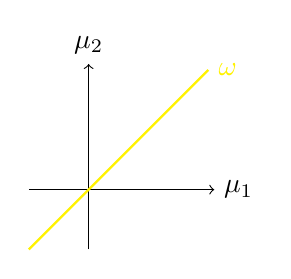
\begin{tikzpicture}[scale=0.38]
  \draw[->] (-2, 0) -- (4.2, 0) node[right] {$\mu_1$};
  \draw[->] (0, -2) -- (0, 4.2) node[above] {$\mu_2$};
	\draw [yellow,thick] (-2,-2) -- (4,4) node [right] {$\omega$};
\end{tikzpicture}
\end{minipage}
\end{frame}
%-------------- end slide -------------------------------%}}}
%-------------- start slide -------------------------------%{{{ 6.43
\begin{frame}
\begin{itemize}
	\item Let $Y_1,\cdots,Y_n$ be a random sample of size $n$ from $f_Y(y;\theta_1,\cdots,\theta_k)$\\[1em]
	\item Let $\Omega$ be all possible values of the parameter vector $(\theta_1,\cdots,\theta_k)$\\[1em]
	\item Let $\omega\subseteq \Omega$ be a subset of $\Omega$.
		\vfill
	\item Test:
		\[
			H_0: \theta\in\omega\quad\text{vs}\quad
			H_1: \theta\in\Omega\setminus\omega.
		\]
		\vfill
	\item The \textcolor{yellow!80!black}{\bf generalized likelihood ratio}, $\lambda$, is defined as
		\[
			\lambda := \frac{\displaystyle \max_{(\theta_1,\cdots,\theta_k)\in\omega} L(\theta_1,\cdots,\theta_k)}{\displaystyle \max_{(\theta_1,\cdots,\theta_k)\in \Omega}L(\theta_1,\cdots,\theta_k)}
		\]
\end{itemize}
\end{frame}
%-------------- end slide -------------------------------%}}}
%-------------- start slide -------------------------------%{{{ 6.44
\begin{frame}

\begin{itemize}
	\item[]
	\begin{align*}
		\lambda\in (\alert{0},\textcolor{green}{1}]
	\end{align*}
	\begin{center}
	% \begin{tabular}{ccc}
	%  $\lambda$ close to \alert{zero} & data are NOT compatible with $H_0$ & \alert{reject $H_0$}\\
	%  $\lambda$ close to \textcolor{green}{one} &  data are compatible with $H_0$ & \textcolor{green}{accept $H_0$}\\
	% \end{tabular}
\begin{minipage}{0.45\textwidth}
	\begin{center}
		$\lambda$ close to \alert{zero} \\
		data NOT compatible with $H_0$ \\
		\alert{reject $H_0$}
	\end{center}
\end{minipage}
\hfill
\begin{minipage}{0.45\textwidth}
	\begin{center}
		$\lambda$ close to \textcolor{green}{one} \\
		data compatible with $H_0$ \\
		\textcolor{green}{accept $H_0$}
	\end{center}
\end{minipage}
	\end{center}
		\vfill
	\item \textcolor{yellow!80!black}{\bf Generalized likelihood ratio test (GLRT)}: Use the following critical region
		\[
			C =\left\{\lambda: \lambda\in(0,\lambda^*]\right\}
		\]
		to reject $H_0$ with either $\alpha$ or $y^*$ being determined through
		\[
			\alpha = \bbP\left(0<\Lambda\le \lambda^*\bigg| \text{$H_0$ is true}\right).
		\]
\end{itemize}
\end{frame}
%-------------- end slide -------------------------------%}}}
%-------------- start slide -------------------------------%{{{ 6.45
\begin{frame}
	Remarks:\\[1em]
	\begin{enumerate}
		\item Maximization over $\Omega$ instead of $\Omega\setminus\omega$ in denominator:
		\item[]		In practice, little effect on this change.
		\item[]	In theory, much easier/nicer: $L(\theta_1,\cdots,\theta_k)$ is maximized over the whole space $\Omega$ by the max. likelihood estimates: $\Omega_e:=(\theta_{e,1},\cdots,\theta_{e,k})\in\Omega$.
			\vfill
		\item Suppose the maximization over $\omega$ is achieved at $\omega_e\in\omega$.
			\vfill
		\item Hence:
			\[
			\lambda = \frac{L(\omega_e)}{L(\Omega_e)}.
			\]
\end{enumerate}
\end{frame}
%-------------- end slide -------------------------------%}}}
%-------------- start slide -------------------------------%{{{ 6.46
\begin{frame}
	Remarks;\\[1em]
	\begin{enumerate}
	\setcounter{enumi}{3}
	\item For simple-vs-composite test, $\omega=\{\omega_0\}$ consists only one point: \\[1em]
			\[
		\lambda = \frac{L(\omega_0)}{L(\Omega_e)}.
			\]
		\vfill
	\item Working with $\Lambda$ is hard since $f_\Lambda(\lambda|H_0)$ is hard to obtain. \\[1em]
	\item[] If $\Lambda$ is a {\it (monotonic) function} of some r.v. $W$, whose pdf is known. \\[1em]
	\item[]
		\begin{center}
		Suggesting testing procedure \\[1em]
		Test based on $\lambda$
		$\quad\Longleftrightarrow\quad$
		Test based on $w$.
		\end{center}
	\end{enumerate}
\end{frame}
%-------------- end slide -------------------------------%}}}
%-------------- start slide -------------------------------%{{{ 6.47
\begin{frame}
	\begin{enumerate}
		\item[E.g. 1] Let $Y_1,\cdots,Y_n$ be a random sample of size $n$ from the uniform pdf: $f_Y(y:\theta)=1/\theta$, $y\in[0,\theta]$. Find the form of GLRT for
			\[
				H_0: \theta=\theta_0\quad\text{v.s.}
				\quad
				H_1:\theta<\theta_0
				\qquad\quad \text{with given $\alpha$.}
			\]
\vfill
\item[Sol.] 1) The null hypothesis is simple, and hence
	\[
		L(\omega_e) = L(\theta_0) = \theta_0^{-n} \prod_{i=1}^n I_{[0,\theta_0]}(y_i)
		=\theta^{-n}I_{[0,\theta_0]}(y_{max}).
	\]
\item[]	2) The MLE for $\theta$ is $y_{max}$ and hence,
	\[
		L(\Omega_e) = L(y_{max}) =
		y_{max}^{-n}I_{[0,y_{max}]}(y_{max})= y_{max}^{-n}.
	\]
	\end{enumerate}
\end{frame}
%-------------- end slide -------------------------------%}}}
%-------------- start slide -------------------------------%{{{ 6.48
\begin{frame}

	\begin{enumerate}
	\item[]	3) Hence,
		\[
			\lambda =
			\frac{L(\omega_e)}{L(\Omega_e)} =
			\left(\frac{y_{max}}{\theta_0}\right)^nI_{[0,\theta_0]}(y_{max})
		\]
	\item[] that is, the test statistic is
			\[
				\Lambda = \left(\frac{Y_{max}}{\theta_0}\right)^n I_{[0,\theta_0]}(Y_{max}).
			\]
			\vfill
	\item[] 4) $\alpha$ and critical value $\lambda^*$:
\begin{align*}
			\alpha & =
			\bbP(0<\Lambda\le \lambda^*| \text{$H_0$ is true})
			\\&=
			\bbP\left(\left[\frac{Y_{max}}{\theta_0}\right]^n I_{[0,\theta_0]}(Y_{max}) \le \lambda^*\bigg| \text{$H_0$ is true}\right)
			\\&=
			\bbP\left(Y_{max}  \le\theta_0 (\lambda^*)^{1/n}\bigg| \text{$H_0$ is true}\right)
		\end{align*}
		\vfill
	\item[] \hspace{2em} $\Lambda$ suggests the test statistic $Y_{max}$:\\[0.5em]
		\[\text{Test based on $\lambda$ $\Longleftrightarrow$ Test based of $y_{max}$}\]
	\end{enumerate}
\end{frame}
%-------------- end slide -------------------------------%}}}
%-------------- start slide -------------------------------%{{{ 6.49
\begin{frame}
	\begin{enumerate}
		\item[] 5) Let's find the pdf of $Y_{max}$. The cdf of $Y$ is $F_Y(y;\theta_0) = y/\theta_0$ for $y\in [0,\theta_0]$. Hence,
			\begin{align*}
				f_{Y_{max}}(y;\theta_0)
				&=n F_Y(y;\theta_0)^{n-1}f_Y(y;\theta_0)\\
				&= \frac{n y^{n-1}}{\theta_0^n},\quad y\in [0,\theta_0].
			\end{align*}
			\vfill
		\item[] 6) Finally, by setting $y^*:= \theta_0(\lambda^*)^{1/n}$, we see that
			\begin{align*}
				\alpha&=
				\bbP\left(Y_{max}  \le y^* \bigg| \text{$H_0$ is true}\right)
				    \\&= \int_0^{y^*} \frac{ny^{n-1}}{\theta_0^n} \ud y
				    \\&= \frac{(y^*)^n}{\theta_0^n} \quad\Longleftrightarrow\quad
				    y^* = \theta_0 \alpha^{1/n}.
			\end{align*}
			\vfill
		\item[]	7) Therefore, $H_0$ is rejected if
			\[
				y_{max}\le  \theta_0 \alpha^{1/n}.
			\]
			\myEnd
	\end{enumerate}
\end{frame}
%-------------- end slide -------------------------------%}}}
%-------------- start slide -------------------------------%{{{ 6.50 Eg. 2
\begin{frame}

	\begin{enumerate}
		\item[E.g. 2] Let $X_1,\cdots,X_n$ be a random sample from the geometric distribution with parameter $p$.
			% \[
				% p_X(k;p) = (1-p)^{k-1}p, \quad k=1,2,\cdots
			% \]
		\item[] Find a test statistic $\Lambda$ for testing
			$H_0 : p = p_0$ versus $H_1 : p \ne p_0$.
			\vfill
		\item[Sol.] Let $\overline{X}$ and $\overline{k}$ be the sample mean. Because the null hypothesis is simple,
	\[
		L(\omega_e) = L(p_0) =  \prod_{i=1}^n  (1-p_0)^{k_i-1}p_0= (1-p_0)^{n \bar{k}-n} p_0^n,
	\]
\item[] which shows that $\bar{k}$ is a sufficient estimator.
\item[] On the other hand, the MLE for the parameter $p$ is $1/\bar{k}$. So
	\[
		L(\Omega_e) = L(1/\bar{k}) = \prod_{i=1}^n \left(1-\frac{1}{\bar{k}}\right)^{k_i-1}\frac{1}{\bar{k}} = \left(\frac{\bar{k}-1}{\bar{k}}\right)^{n\bar{k}-n} \frac{1}{\bar{k}^{n}}.
	\]
\item[]	Hence,
	 \[\lambda=\frac{L(\omega_e)}{L(\Omega_e)}
	 = \left(\frac{\bar{k}(1-p_0)}{\bar{k}-1}\right)^{n\bar{k}-n} (p_0 \bar{k})^n\]
 \item[] Finally, $\Lambda= \left(\frac{\overline{X}(1-p_0)}{\overline{X}-1}\right)^{n\overline{X}-n} (p_0 \overline{X})^n$. \myEnd
	\end{enumerate}
\end{frame}
%-------------- end slide -------------------------------%}}}
%-------------- start slide -------------------------------%{{{ 6.51 Eg 3
\begin{frame}

\begin{enumerate}
		\item[E.g. 3] Let $Y_1,\cdots,Y_n$ be a random sample from the exponential distribution with parameter $\lambda$.
		\item[] Find a test statistic $V$ for testing $H_0 : \lambda = \lambda_0$ versus $H_1 : \lambda \ne \lambda_0$.
			\vfill
		\item[Sol.]Since the null hypothesis is simple,
			\[
				L(\omega_e) = L(\lambda_0)  = \prod_{i=1}^n \lambda_0e^{-\lambda_0 y_i} = \lambda_0^n e^{-\lambda_0 \sum_{i=1}^n y_i}
			\]
		\item[] Let $Z=\sum_{i=1}^n Y_i\sim$ Gamma$(n,\lambda)$, which is a sufficient estimator.
		\item[] On the other hand, the MLE for $\lambda$ is $1/\bar{y}=n/z$:
			\[
				L(\Omega_e) = L(1/\bar{y}) = (n/z)^{n} e^{-n}.
			\]
	 \item[] Hence,
		 \[
			 \lambda =\frac{L(\omega_e)}{L(\Omega_e)} = z^nn^{-n} \lambda_0^n e^{-\lambda_0 z+n}
		 \]
 \item[] Finally, $\Lambda=Z^nn^{-n} \lambda_0^n e^{-\lambda_0 Z+n} $\qquad \pause or \qquad $V = Z^n e^{-\lambda_0 Z}$. \myEnd
	\end{enumerate}
\end{frame}
%-------------- end slide -------------------------------%}}}
%-------------- start slide -------------------------------%{{{ 1
\begin{frame}[fragile]
\begin{itemize}
	\item[] The critical region in terms of $V$ should be:
	\begin{align*}
		0.05 = \alpha & = \bbP\left(V\in(0,y^*]\bigg|\text{$H_0$ is true}\right)\\
		& = \int_0^{y^*} f_V(v)\ud v
	\end{align*}
	\item[] However, it is not easy to find the exact distribution of $V$.
	\vfill
	\item[] One can also make the inference based on the test statistic $Z$ ...
	\end{itemize}
\end{frame}
%-------------- end slide -------------------------------%}}}
%-------------- start slide -------------------------------%{{{ 1 v(z) function plot
\begin{frame}[fragile]
\begin{center}
	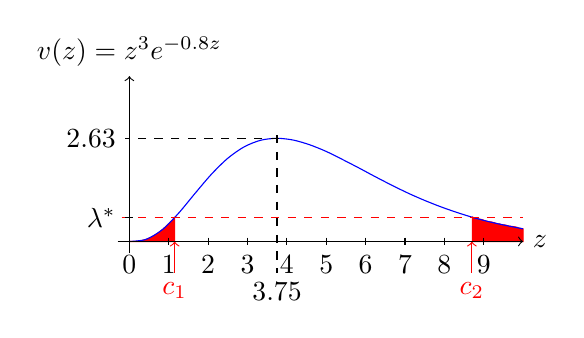
\begin{tikzpicture}[scale=0.5]
  % \filldraw[scale=1, domain=3.7:3.8, smooth, variable=\x, green] plot ({\x}, {\x*\x*\x*exp(-0.8*\x)}) -- (3.8,2.6248) -- (3.7,2.6248);
	\def\left{1.15}
  \filldraw[scale=1, domain=0:\left, smooth, variable=\x, red] plot ({\x}, {\x*\x*\x*exp(-0.8*\x)}) -- (\left,0) -- (0,0);
	\def\right{8.7}
  \filldraw[scale=1, domain=\right:10, smooth, variable=\x, red] plot ({\x}, {\x*\x*\x*exp(-0.8*\x)}) -- (10,0) -- (\right,0);
  \draw[scale=1, domain=0:10, smooth, variable=\x, blue] plot ({\x}, {\x*\x*\x*exp(-0.8*\x)});
	\foreach \x in {0,...,9}{
			\draw (\x,0.1)--++(0,-0.2) node [below] {$\x$};
	}
	\draw[dashed] (3.75,2.7) -- (3.75,-0.8) node [below] {$3.75$};
	\draw[dashed] (3.8,2.6255) -- (-0.1,2.6255) node [left] {$2.63$};
	\def\level{0.6}
	\draw[dashed,red] (-0.2,\level) -- (10,\level);
	\draw[red,<-] (\left,0) -- (\left, -0.8) node [below] {$c_1$};
	\draw[red,<-] (\right,0) -- (\right, -0.8) node [below] {$c_2$};
	\draw (-0.1,\level) node [left] {$\lambda^*$} -- (0.1,\level);
  \draw[->] (-0.3, 0) -- (10, 0) node[right] {$z$};
  \draw[->] (0, -0.3) -- (0, 4.2) node[above] {$v(z)=z^3e^{-0.8z}$};
	\end{tikzpicture}

	\vfill

	This suggests that the critical region in terms of $z$ should be of the form:
	\begin{align*}
		(0,c_1) \cup (c_2,\infty)
	\end{align*}
	For convenience, we put $\alpha/2$ mass on each tails of the density of $Z$:\\[1em]
	Find $c_1$ and $c_2$ such that
	\begin{align*}
		\int_0^{c_1} f_{Z}(z)dz = \int_{c_2}^\infty f_{Z}(z)dz = \frac{\alpha}{2}.
	\end{align*}
\end{center}
\end{frame}
%-------------- end slide -------------------------------%}}}
%-------------- start slide -------------------------------%{{{ 1
\begin{frame}[fragile]
\begin{center}

	\renewcommand{\arraystretch}{2}
	\begin{tabular}{c|cc}
                  & using $V$      & using $Z$                  \\ \hline
	Critical region & $(0,v^*]$      & $(0,z_1]\cup [z_2,\infty)$ \\
	pdf             & hard to obtain & Gamma $(n,\lambda)$        \\
	\end{tabular}
\end{center}
\end{frame}
%-------------- end slide -------------------------------%}}}
%-------------- start slide -------------------------------%{{{ 6.52 Eg. 4
\begin{frame}

	\begin{enumerate}
		\item[E.g. 4] Let $Y_1,\cdots,Y_n$ be a random sample from $N(\mu,1)$.
		\item[] Find a test statistic $\Lambda$ for testing $H_0 : \mu = \mu_0$ versus $H_1 : \mu \ne \mu_0$.
			\vfill
		\item[Sol.]Since the null hypothesis is simple,
\[
	L(\omega_e) = L(\mu_0) = \prod_{i=1}^n\frac{1}{\sqrt{2\pi}}e^{-\frac{(y_i-\mu_0)^2}{2}}.
\]
\item[] On the other hand, the MLE for $\mu$ is $\bar{y}$:
	\[
	L(\Omega_e) = L(\bar{y}) =
	\prod_{i=1}^n\frac{1}{\sqrt{2\pi}}e^{-\frac{(y_i-\bar{y})^2}{2}}.
	\]
\item[] Hence,
\[	 \lambda=\frac{L(\omega_e)}{L(\Omega_e)}
	 = \exp\left(-\sum_{i=1}^n \frac{(y_i-\mu_0)^2 -(y_i-\bar{y})^2}{2}\right)
	 = \exp\left(-\frac{n (\bar{y}-\mu_0)^2}{2}\right).
\]
 \item[] Finally, $\Lambda= \exp\left(-\frac{n}{2} \left(\overline{Y}-\mu_0\right)^2
	 \right)$\pause\qquad or\qquad $V =  \frac{\overline{Y}-\mu_0}{1/\sqrt{n}}\sim N(0,1)$ \myEnd
	\end{enumerate}
\end{frame}
%-------------- end slide -------------------------------%}}}

\end{document}

